\documentclass{mcmthesis}
\mcmsetup{CTeX = false,   % 使用 CTeX 套装时,设置为 true
        tcn = 2108321, problem = C,
        sheet = true, titleinsheet = true, keywordsinsheet = true,
        titlepage = false, abstract = false}
\usepackage{palatino}
\usepackage{lipsum}
\usepackage{float}
\usepackage{geometry}
%===============设置正文和数学字体=============================
%有些字体需要安装一些字体文件,注意辨别。
%我参照 MCM论文集的字体 使用如下宏包来定制字体。

\usepackage{graphicx}

\usepackage{subfigure}
%设置段落之间的距离,若不需要删除或者注释掉即可。
\setlength\parskip{.5\baselineskip}
\newtheorem{definition}{Definition}[section]
%\def\abstractname{Summary}%可修改摘要名称
\usepackage{url}
\usepackage{indentfirst}
\setlength{\parindent}{2em}
\usepackage{siunitx}
\usepackage{chngpage}
\usepackage{array}
\usepackage{booktabs}
\usepackage{threeparttable}
\usepackage{longtable}
\usepackage[numbers,sort&compress]{natbib}
\usepackage{amsmath}
\numberwithin{figure}{section}
\numberwithin{table}{section}
%%% 实现参考文献标号在右上角
\newcommand{\upcite}[1]{\textsuperscript{\textsuperscript{\cite{#1}}}}
%然后引用的时候使用\upcite{}的格式(一般的正常引用格式为\cite{})



\usepackage{titletoc}
\titlecontents{section}[3cm]{\bf \large}{\contentslabel{2.8em}}{}{%
\titlerule*[0.5pc]{$\cdot$}\contentspage}%
\titlecontents{subsection}[4cm]{\normalsize}{\contentslabel{2.5em}}{}{%
\titlerule*[0.5pc]{$\cdot$}\contentspage}%
\titlecontents{subsubsection}[5.3cm]{\normalsize}{\contentslabel{3.0em}}{}{%
\titlerule*[0.5pc]{$\cdot$}\contentspage}%



\title{\large The Prediction to the Migration of Scottish Herring and Mackerel }
\author{}
\date{\today}
\geometry{left=2.5cm,right=2.5cm}

\begin{document}



\begin{abstract}
  This paper establishes a model for the spread of Vespa mandarinia over time and a priority assessment model for eyewitness reports. By analyzing the notes, pictures, and sighting locations provided by the eyewitnesses, the multimodal classification model established in this paper is able to lead to prioritizinginvestigation of the reports most likely to be positive sightings.
  
  For the spread of Vespa mandarinia over time , this paper analyzed the distribution of honey bee hives, vegetation cover, hornet habits, and rated the risk for each county in Washington. This paper then inferred three possible spread routes of hornet and a key area for hornets. For the priority assessment model of eyewitness reports, this paper uses three sub-classification models to obtain the final multimodal classification model, which specifically includes a risk assessment model based on the location of the sighting, a note classification model based on Naive Bayes, and a picture classification model based on EfficientNet. In this paper, the original data are firstly preprocessed with formatting, data enhancement, sample equalization,  training set slicing, and then the three sub-models are trained independently. Finally the hyperparameters of model fusion are analyzed for sensitivity. Considering the existence of many unlabeled samples, this paper uses a semi-supervised approach to train the models. Considering the dynamic expansion of samples, this paper suggests using batch learning to update the model when the number of new samples reaches 400.
  
  This paper prioritizes the Unprocessed and Unverified labeled samples and lists the top eight samples in terms of likelihood of Vespa mandarinia occurrence. This paper summarizes the advantages and disadvantages of the model, and puts forward the future improvement work.
  
\begin{keywords}
EfficientNet; Naive Bayes; Semi-supervision; Batch Learning  

\end{keywords}
\end{abstract}
\maketitle
\pagestyle{empty}
\newpage                                                          %
%==================================================================
%====================生=成=目=录===================================
\begin{adjustwidth}{-1cm}{0cm}

\setcounter{tocdepth}{3}
\thispagestyle{empty}
\tableofcontents                                                  %

\end{adjustwidth}


\newpage

\pagestyle{fancy}

\setcounter{page}{1}
\section{Introduction}
\subsection{Background}

The Asian giant hornet is the largest and most cruel hornet in the world. It looks like a AA battery with wings and armor. It also has a huge stinger and eagers to bite off the bee’s head and sting people. The name "killer bumblebee" comes from this giant insect that can kill the entire bee colony, and the deaths of dozens of people each year are also related to them.

What makes people worried is that North American bees do not know how to fight back Asian giant hornet like Asian bees. Asian bees will use a strategy called "hotball" to kill Asian hornet. This strategy means that Asian honeybees will swarm on a Asian giant hornet that is much larger than them and begin to vibrate their small bodies, producing enough heat to effectively "cook" the hornet from within, thereby killing it. Experts worry that Vespa mandarinia hornet may have catastrophic consequences for European bees in North America. The number of European honeybees in North America was reduced due to pesticides and many other factors. Now such a huge enemy has been added.

Considering the huge threat of the Asian giant Hornet, it is particularly important for the Washington Department of Agriculture to take precise measures to eliminate it. Therefore, the Washington State Department of Agriculture said in a statement: “The most likely time to catch the Asian giant Hornet is from July to October. This is when the colony is established and the workers are foraging. If you want to trap the queen, the earliest the trap can be hung in April, but because the number of queens is significantly less than the workers, the possibility of catching the queen is very small." These researchers are working with the Washington State Department of Agriculture, beekeepers and the public to find and study these giant hornets, and prevent its spread.

This article discusses the spread of Asian giant hornets over time and hopes to help the Washington Department of Agriculture deal with more urgent reports by predicting the probability of this sighting being a Vespa mandarinia based on pictures, notes, sighting locations, time and other information reported by witnesses.


\subsection{Problem Analysis}

% 问题一:建立一个数学模型,以确定这两种鱼类在未来50年内最有可能出现的位置,假设水温变化足以导致种群移动。

% 问题二:根据海水温度变化,使用您的模型预测最佳情况和最坏情况,到时这些小渔业公司因距离鱼群太远将无法收获。

% 问题三:根据你的预测分析,这些小型渔业公司是否应该改变他们的经营?

% a、如果是,请使用您的模型来确定和评估对小型渔业公司具有实际和经济吸引力的战略。你的策略应该考虑但不限于现实的选择,包括:

%  -将渔业公司的部分或全部资产从苏格兰港口的当前位置转移到更靠近两个鱼类种群移动的位置;

% -使用一定比例的小型渔船,可以在没有陆地的情况下作业一段时间,同时仍然确保渔获物的新鲜度和高质量。

% b、如果您的团队拒绝任何更改的需要,请根据您的建模结果证明您拒绝的原因,因为它们与您的团队所做的假设有关。

% 问题四:如果某一比例的渔业进入另一个国家的领海(海洋),请使用您的模型来说明您的方案受到的影响。

% 问题五:除了你的技术报告外,为相关组织准备一到两页的文章,以帮助渔民了解问题的严重性,以及你提出的解决方案将如何改善他们未来的商业前景。
\begin{itemize}
  \item \textbf{Address and discuss whether or not the spread of this pest over time can be predicted,and with what level of precision.}
  
First, we analyze the living habits and determine the suitable living environment of Vespa mandarinia. Then we comprehensively consider the distribution of bee hives in each county in Washington State, vegetation coverage, traffic topography and other factors, and score the basic situation of each county in Washington State. Combining these objective factors and a small amount of wasp sighting samples, we can easily analyze the distribution of this pest over time. Considering that the number of positive samples is less than 20 and the distribution area is very cramped, we can roughly divide the key areas of Asian giant hornet distribution and the possible migration routes over time. The accuracy of the model can be measured by analyzing the number of positive samples that fall in the area.
  
  \item \textbf{Most reported sightings mistake other hornets for the Vespa mandarinia. Use only the data set file provided, and (possibly) the image files provided, to create, analyze, and discuss a model that predicts the likelihood of a mistaken classification.}

Most of the samples were mistaken as Vespa mandarinia by eyewitnesses, and these samples wereted a lot of staff confirmation time. Therefore, it is necessary to determine the priority of the report through the pictures, notes, sighting location, time and other information provided in the eyewitness report. For this multi-modal binary classification model, we obtain the report priority through the weighted fusion of the three sub-classification models. Specifically, we use EfficientNet to complete the two classification of images, use Naive Bayes to complete the two classification of notes, and use the risk assessment model to complete the two classification of sighting locations. 
  
First, we format the original data, clean the data, and then segment the data according to different sub-model requirements. In addition, it is necessary to appropriately expand the positive samples to solve the problem of sample imbalance. For the picture classification model, data enhancement is also needed to enhance the robustness of the model. For pictures with more unprocessed and unverified tags, a semi-supervised learning method is used to complete the two classification in the iterative process. Finally, we sum up the scores of the three sub-models as the final score.


  \item \textbf{Use your model to discuss how your classification analyses leads to prioritizing investigation of the reports most likely to be positive sightings.}

The output of our model represents the priority level of the report. If it is higher than a certain threshold, the staff should give priority to it. The score priorities of the three sub-models are different. The image classification model has the highest priority, the sighting location risk assessment model is the second, and the comment classification model has the lowest priority.

  \item \textbf{Address how you could update your model given additional new reports over time, and how often the updates should occur.}
  
The number of reports that can be used for training will gradually increase over time. In order to ensure that the performance of the model can continue to improve, we need to update the model in the manner of batch learning when the number of new samples reaches 400, about 20 days.

  \item \textbf{Using your model, what would constitute evidence that the pest has been eradicated in Washington State?}

We use our model to evaluate the priority of reports with unprocessed and unverified labels. If all priority of reports are lower than the default threshold and combining the living habits of the Vespa mandarinia, we can infer that the Asian giant hornet has been eradicated in Washington State with the statistical law.

\end{itemize}


\section{Assumptions and Symbols Definitions}
\subsection{Assumptions}

\begin{itemize}
\item It is assumed that that the data is true and valid and the source is reliable.

\item It is assumed that the migration of Vespa mandarinia over time is completely determined by its living habits and environment.

\item It is assumed that every position of Asian giant hornet can be immediately discovered by witnesses.


\item It is assumed that the manually constructed positive sample and the real sample have the same distribution.


\item It is assumed that the fusion model can always break through the data bias of a single model.


\end{itemize}


\subsection{Symbols Definitions}

\begin{center}
\begin{longtable}{p{.1\textwidth}p{.8\textwidth}m{.4\textwidth}}
\caption{The List of Notation}\\
\hline
Symbol& Meaning \\
\hline

$A$      & A eyewitness location-based Risk assessment model
                                                         \\
$B$      & A Plain Bayesian-based Notes Classification Model
                                                          \\
$C$     & A EfficientNet-based Picture Classification Model
                                                        \\
$D$       & The fusion model of the above three single models                                                       \\
$S_i$      & The priority score of model i, the value range is $0 \sim 1$, 1 corresponds to the highest priority
                                                            \\
$(x_0,y_0)$       & The center coordinate of the key area
                                 \\
$r_0$       & The radius of the key area
                                         \\
$(x,y)$       & The sighting location, x represents latitude and y represents longitude
\\
$r$       & The distance from the sighting location to the center of key area \\
$F_1$       & The risk score based on the distance from the key area, the value range is $0 \sim 1$, 1 corresponds to the highest risk level \\
$F_2$      &  The risk score based on the number of bee hives and vegetation coverage, the value range is $0 \sim 1$, 1 corresponds to the highest risk level
\\
$\gamma$      &  The weight of $F_1$ in model A, the range is $0 \sim 1$

\\
$\alpha$       & The weight of model A in model D, the range is $0 \sim 1$

\\
$\beta$       & The weight of model B in model D, the range is $0 \sim 1$
\\
$1-\alpha-\beta$       & The weight of model C in model D, the range is $0 \sim 1$
\\
                                                        \\ \hline

 \end{longtable}
 \end{center}


\section{Establishment and Solution of Model}
\subsection{Modeling changes in the distribution of Asian hornets}

The life cycle of an Asian giant hornet begins with a queen’s nest building after overwintering. During this period, the queen develops a nest, collects and eats arthropods and sap, and prepares to lay eggs. The colony begins in summer, the queen takes care of her cubs, and worker ants finally begin to appear. Once the queen has produced enough workers, the responsibility of predation is completely transferred to the workers, and the queen stays in the nest to continue laying eggs.


In order to estimate the risk of Asian giant hornet to Washington, we have carried out a risk rating for each county in Washington. The reference standards are as follows: 
\begin{enumerate}
  \item Winter climate suitability
  \item Whether the habitat is suitable for Asian giant hornet colonization nests (This is based on the dense forest biomass)
  \item The hive density of the counties
  \item The path (main port or freight hub) that may introduce Asian Hornet
\end{enumerate}

Because the prey objects of Asian giant hornet are mainly honeybees, and the nesting and reproduction of Asian giant hornet are inseparable from trees and vegetation, we recommend that the Washington government pay more attention to counties with a large number of hives, extensive vegetation coverage, and convenient transportation. We consulted relevant information \cite{REF1} and sorted out the number of hives and vegetation coverage in each county in Washington. The following figure shows the corresponding data:



\begin{figure}[H]
  \centering{
  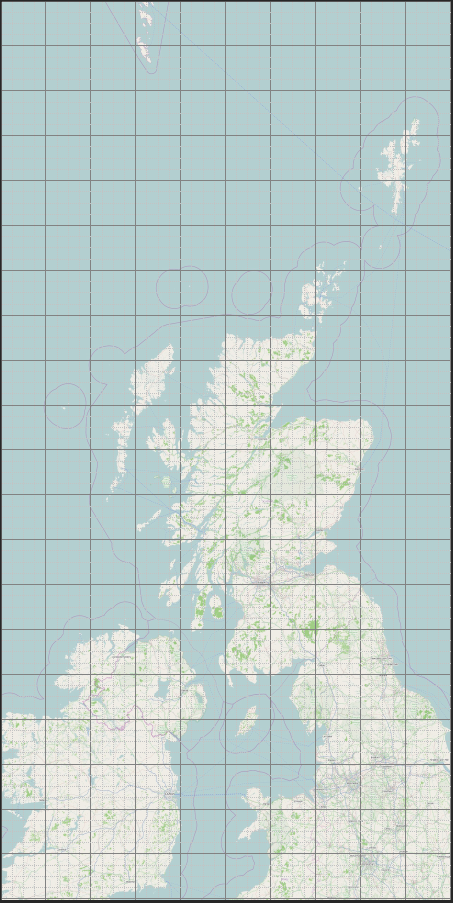
\includegraphics[width=12cm]{./picture/1_1.png}}
  \caption{Total hives of each county in Washington}\label{1_1}
\end{figure}

\begin{figure}[H]
  \centering{
  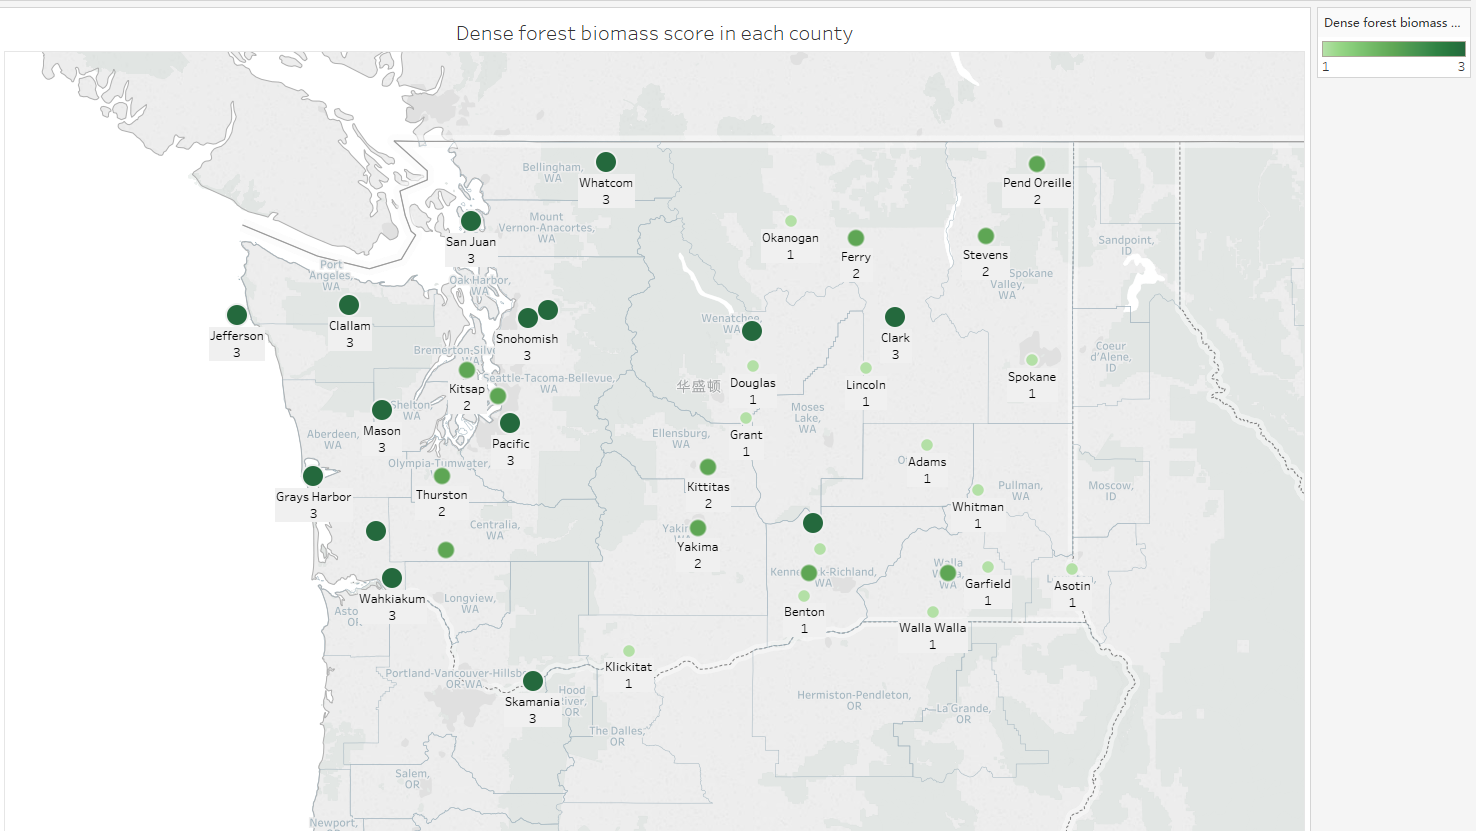
\includegraphics[width=12cm]{./picture/1_2.png}}
  \caption{The dense forest biomass score of each county in Washington}\label{1_2}
\end{figure}

From the above two pictures, we can check the number of hives and the level of vegetation coverage in each county. In addition, we need to consider the county’s transportation convenience level and winter climate comfort. After considering these standards, we will sum up the scores in these four categories and the final score obtained is the risk grade score of the county (appendix quoted table). So far, we can give a risk score to each location in Washington State, and the score only depends on the above four criteria for that location. We denote the risk score of the location of latitude $x$ degrees and longitude $y$ degrees as $F_1(x,y)$.

We combined the above analysis to discuss the distribution of Asian giant hornet over time. We collected information about 14 samples of Asian giant hornet sightings from the official website of the Washington Department of Agriculture (cited), and began to analyze the relevance of the samples. First of all, most of the sighting reports received by the government are not the Asian giant Hornet. We can easily find that the emergence of the Asian Hornet is controlled in a very small area. This may be attributed to the timely and effective measures taken by the government. Secondly, analyzing the time of sightings of the Asian giant Hornet, we can roughly find several earlier positions of the Asian giant Hornet, all of which were before June 2020. The four sighting samples are :
% make a table
\begin{figure}[H]
  \centering
  \subfigure[After 10 years]{               %小图题的名称
  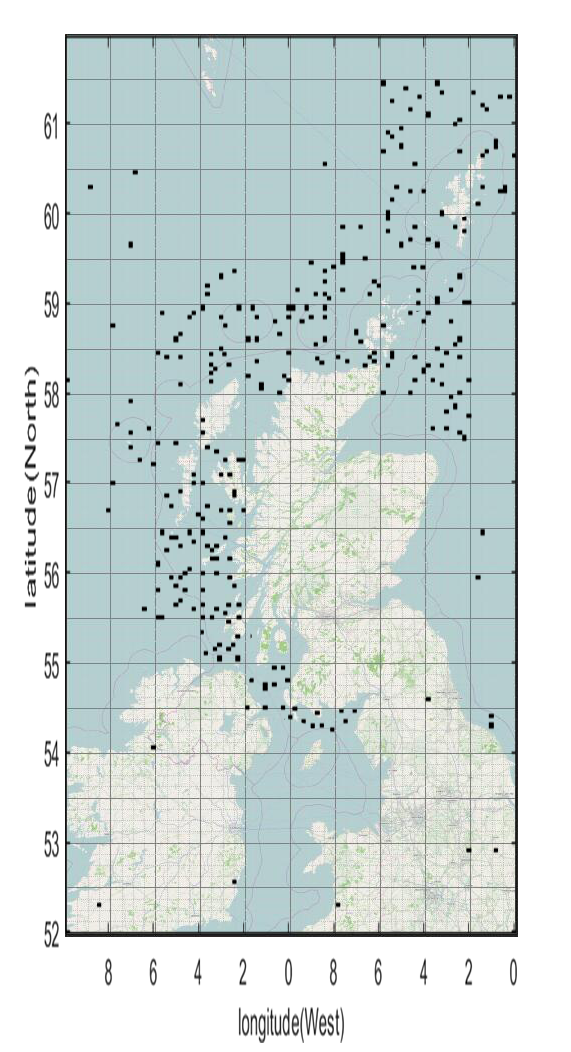
\includegraphics[width=4cm]{./picture/1_10.png}}
  \hspace{0in}
  \subfigure[After 20 years]{
  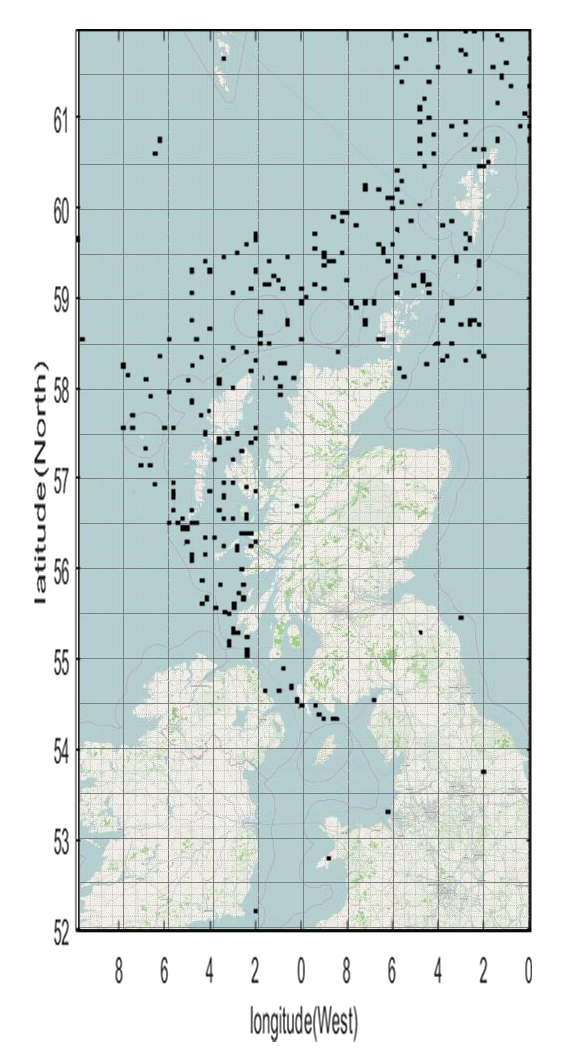
\includegraphics[width=4cm]{./picture/1_11.png}}
  \hspace{0in}
  \subfigure[After 30 years]{
  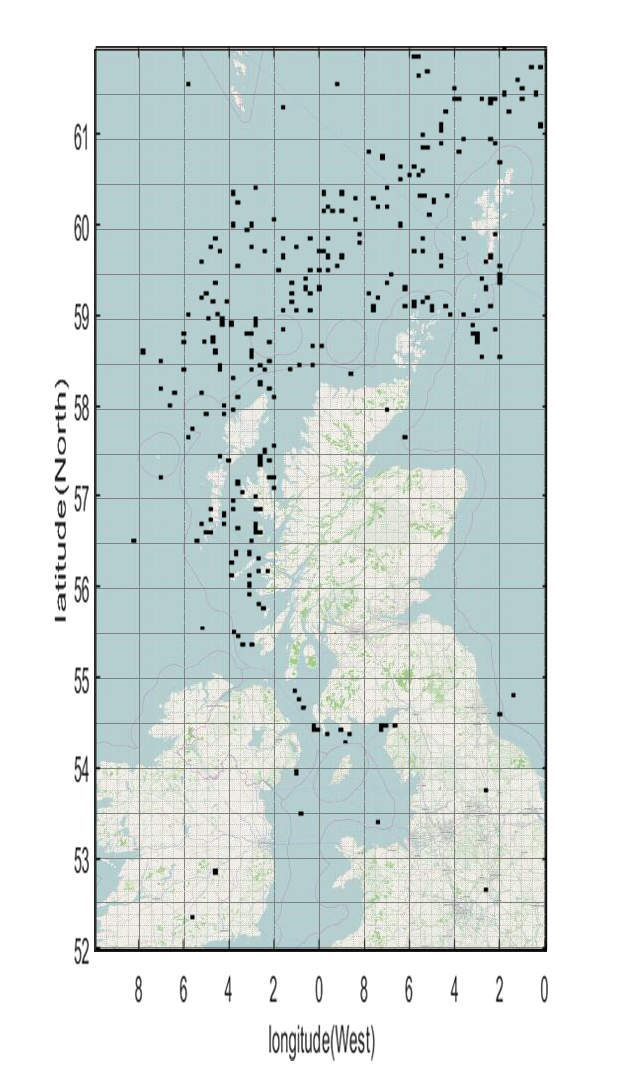
\includegraphics[width=4.2cm]{./picture/1_12.png}}
  \hspace{0in}
  \subfigure[After 40 years]{
  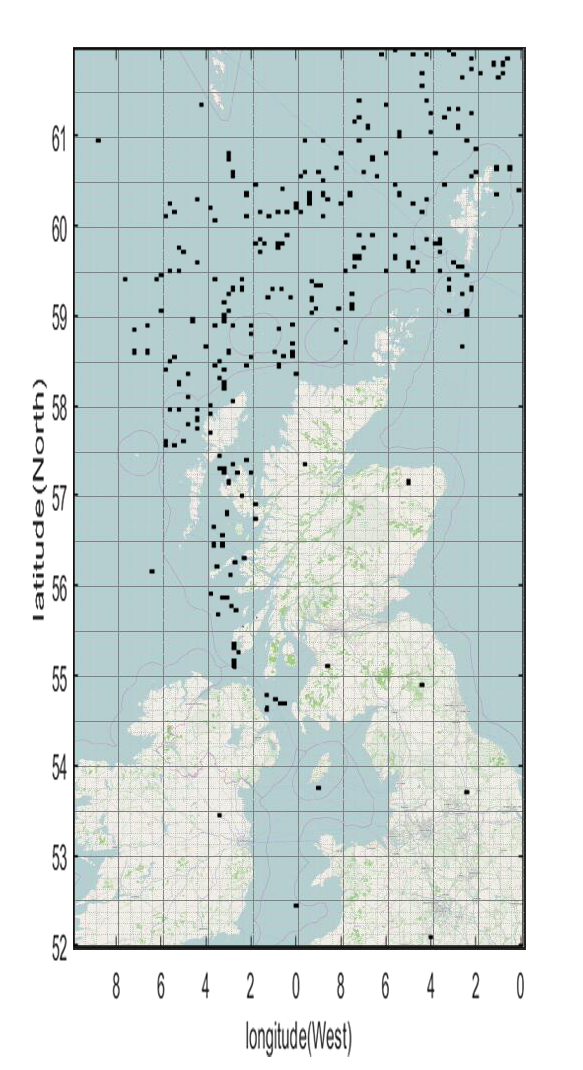
\includegraphics[width=4cm]{./picture/1_13.png}}
  \hspace{0in}
  \subfigure[After 50 years]{
  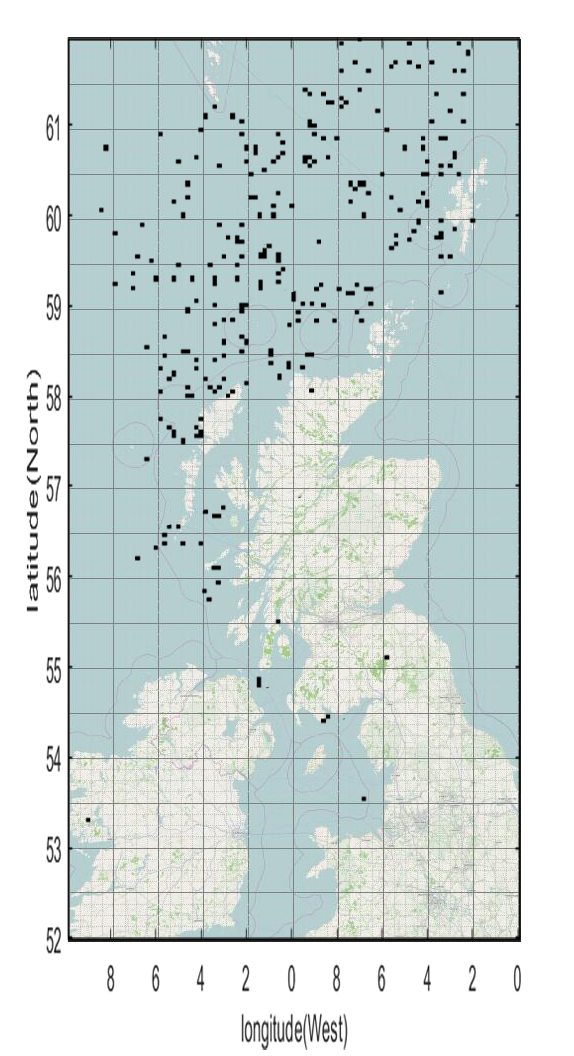
\includegraphics[width=4cm]{./picture/1_14.png}}
  \label{Dist}
  \caption{The prediction of future fish school distribution around Scotland}
  \end{figure}


\begin{figure}[H]
  \centering{
  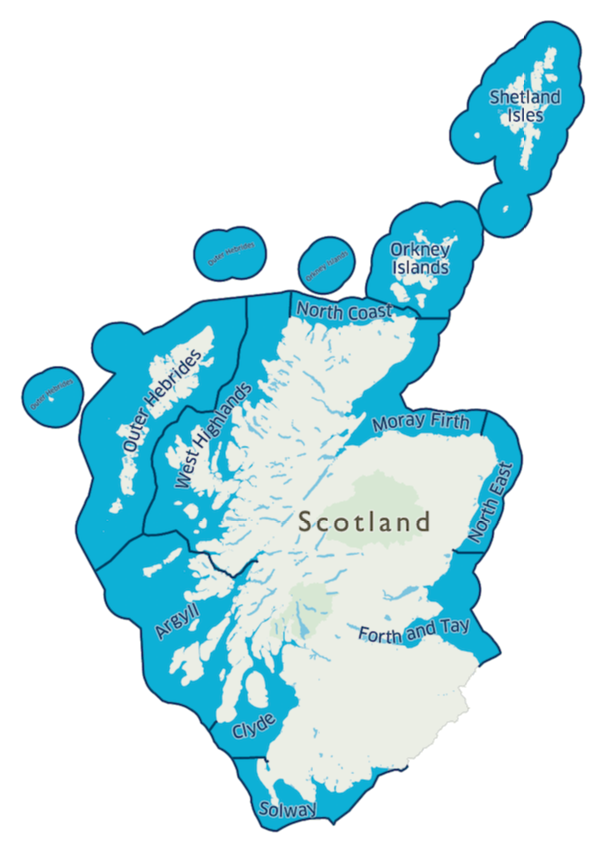
\includegraphics[width=3cm]{./picture/1_3_1.png}}
  \caption{Fisheries around Scotland}\label{FisheriesAround}
\end{figure}

\begin{table}[H]
\centering
\begin{tabular}{|l|l|}% 通过添加 | 来表示是否需要绘制竖线
\hline  % 在表格最上方绘制横线
\textbf{Fishery Name}&\textbf{Representative Color}\\
\hline  %在第一行和第二行之间绘制横线
Argyll \& Clyde & Brown\\
\hline % 在表格最下方绘制横线
Orkney Islands & Yellow\\
\hline % 在表格最下方绘制横线
Outer Hebrides  & Purple\\
\hline % 在表格最下方绘制横线
Shetland Isles & Blue\\
\hline % 在表格最下方绘制横线
North Coast \& West Highlands & Green\\
\hline % 在表格最下方绘制横线
\end{tabular}
\caption{Represntive Color of Fisheries}
\label{FisheryColor}
\end{table}

Then we analyzed the neighborhood relationship between the sighting lFocations of the Asian giant Hornet and found that in the north of San Juan County and in the  of west of Whatcom County, a circular key area was formed. This area is obviously a dense area for Asian giant Hornet sightings. The sighting time of the Asian giant Hornet is probably from September to November 2020. In order to facilitate subsequent processing, we simplify the area to a circle with a radius of $r_0$. Finally, we analyzed the possible migration paths of the Asian giant Hornet. Considering that the road transportation in the key area is more convenient and close to the sea, we infer that the scattered Asian Hornet sightings around the key area may have migrated from the key area. The analysis process of the distribution changes of the Vespa mandarinia over time can refer to the following figure.



\begin{figure}[H]
  \centering{
  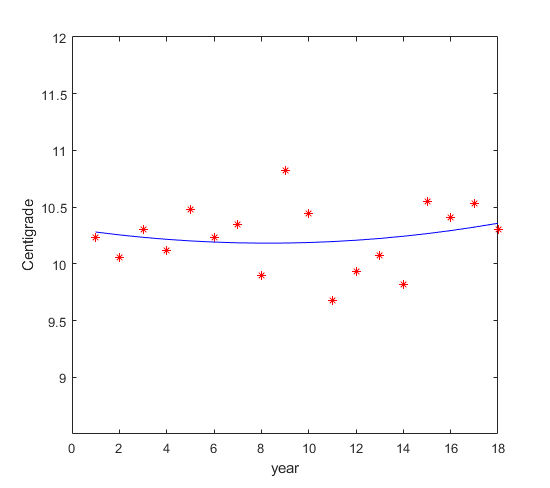
\includegraphics[width=10cm]{./picture/1_4.png}}
  \caption{Schematic diagram of the direction of the Asian Hornet}\label{1_4}
\end{figure}

The blue areas are the earlier areas, but the Asian giant Hornet samples in two blue areas were cleared at the beginning. The red circular area at the border of  Washington State and Canada is the key area with the most reports of Asian giant Hornet sightings. The three black arrows indicate the possible migration routes of Asian giant hornet. The scattered reports may have been migrated by Asian giant hornet in the key area. 

The accuracy of the model can be measured by analyzing the number of positive samples that fall in the key area. We can easily observe that there are 10 points that fall in the red circular area in the above figure. These 10 points occupy more than half of all 18 red points. Our model can accurately reflect the migration trend of Vespa mandarinia.

\subsection{Sighting Report Priority Assessment Model}
\subsubsection{A risk assessment model based on the location of the sighting}
In the above distribution model over time, we can see that sighting location do help us determine the risk rating of the report. Next we will specifically explain the risk assessment model based on the reported sighting location. We believe that the score of this sub-model is a weighted score of the distance to the key area and the risk rating score of the county. In order to simplify the processing, we use the following formula to express:

\begin{equation}
    S_{A(x,y)} = \gamma F_1(x,y)+ (1-\gamma) F_2(x,y)
\end{equation}

The score of model A at position (x, y) should be weighted by F1 score and F2 score according to the coefficient gamma. 

Among them, F1 is calculated from the distance from the sighting position to the key area, and the calculation formula is as follows:

\begin{equation}
  F_1 = \begin{cases}
    1 & (x-x_0)^2 + (y - y_0)^2 \leq r_{0}^2 \\
    \frac{r_{0}^2}{(x-x_0)^2+(y-y_0)^2} & (x-x_0)^2 + (y-y_0)^2 > r_{0}^2

  \end{cases}
\end{equation}

We simplify the key area to be a circle with $(x_0, y_0)$ as the center and $r_0$ as the radius. The cluster center of Asian giant hornet appearance address is $(x_0, y_0)=(48.99385, -122.6933)$, the radius of the circle $r_0=0.16822856475640974$. When the sighting location  $(x, y)$ falls within the circular area, the value of $F_1$ is 1, which represents the highest risk at this time; when the sighting location $(x, y)$ falls outside the circular area, $F_1$ is an inverse proportional function between the value and the distance. 

The $F_2$ score is determined by the county's risk rating score. In the distribution change model of the Asian giant Hornet, we have checked the number of hives and vegetation coverage in each county, and scored the risk for each county. Therefore, we can directly find the risk score of the county where $(x,y)$ is located, and use it as the $F_2$ score. 

Now for any witness’s report, we can enter the witness location to get the score of the risk assessment model directly, and it will be fused with the following two sub-models.

\subsubsection{A Plain Bayesian-based Review Classification Model}

According to the existing notes, we can see that all reports that were finally identified as positive do not have a specific description of the appearance, while many of the cases of negative and unverified have detailed description about pests. We can conclude that notes are not significant for whether the sighting is an Asian giant Hornet or not, so the notes classification model based on Naive Bayes has the lowest proportion in the fusion model. But it's not saying that these notes are worthless. In negative reports, the most frequently appearing words are often the Asian giant Hornet characteristics that are most misleading. Therefore, based on this, we can use the frequency of high-frequency misleading words to reversely evaluate the probability that witnesses misjudge the Asian giant Hornet report.

\subsubsection{The Result of Modeling}
First, we calculated the number of fish in each area in the next 50 years based on the sea temperature change model and computer simulation, as shown in Figure\ref{FishProductionCurve}

\begin{figure}[tbp]
  \centering{
  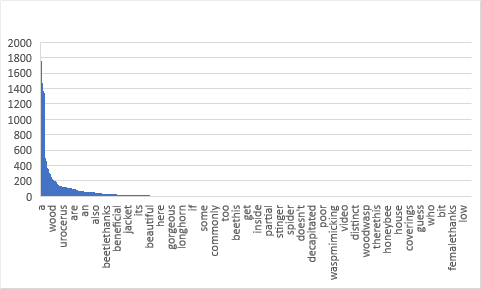
\includegraphics[width=8cm]{./picture/2_1.png}}
  \caption{Fish production curve in each fishery around Scotland within 50 years}\label{FishProductionCurve}
\end{figure}

\begin{table}[!htbp]
  \centering
  \begin{tabular}{|r|c|c|c|c|c|}% 通过添加 | 来表示是否需要绘制竖线
  \hline  %在第一行和第二行之间绘制横线
   & \textbf{Argyll} & \textbf{Orkney} & \textbf{Outer} & \textbf{Shetland} &\textbf{North}\\
  \hline % 在表格最下方绘制横线
  2017 & 70 &35 &32&40&88\\
  \hline % 在表格最下方绘制横线
  2030 & 57&32&26&31&78\\
  \hline % 在表格最下方绘制横线
  2040  & 54&30&28&21&69\\
  \hline % 在表格最下方绘制横线
  2050 &28&19&32&24&56\\
  \hline % 在表格最下方绘制横线
  2060 &22&24&39&25&42\\
  \hline % 在表格最下方绘制横线
  2070 &8&19&35&31&31\\
  \hline % 在表格最下方绘制横线
  \end{tabular}
  \caption{Fish production matrix in each fishery around Scotland within 50 years}
  \label{FisheryTable}
  \end{table}

We found that the fish production of most fisheris is decreasing year by year, and it is related to the geographical location of the fisheris: the latitude of the fishery , the depth of the water area, whether there are other fisheris near the low latitudes and  whether the location is necessary for fish migration all affect the change of fish production in the fishery. We adjusted the parameters in the model to simulate the most likely situation, and the result is as the figure above.

At best, 50 years later, the Argyll \& Clyde fishing grounds in Scotland are the first to fail to harvest.

Assuming that the fish production of a certain fishery is lower than 20\% of the initial production, we regarde that the area will not be able to harvest. According to the statistical results, the production of southest fishery Argyll \& Clyde is less than 20\% of its initial value after about 50 years. From this we can see that if the Argyll \& Clyde fishery does not change its business strategy, its performance will continue to decline and eventually unable to operate. It can be observed from the figure that when the Argyll \& Clyde fishery is facing a crisis, the production of the Outer Hebrides fishery and the Shetland Isles fishery has increased slightly, indicating that some of the fish migrating to the north of the Argyll \& Clyde fishery have entered a certain area in the north, which is a better situation.

At worst, most fisheries, including Shetland Isles, will not be harvested after 200 years.

Based on the trend of global temperature warming and the data of the average sea temperature change in the sea area near Scotland in the past 5 years, we can conclude that the growth rate of its water temperature is increasing year by year. We have to consider the worst case, that is, almost all small fishing companies have no fish to be harvested. Based on this situation, we have adjusted the model parameters of seawater temperature changes to comply with the trend of accelerated global warming and extended the forecast time. In the previous model, we knew that every 20 years, the school of fish moved north by one latitude. Based on the adjusted model, we used the estimated method to get the worst case: 200 years later, most fisheries, including Shetland Isles, will not be harvested.

\subsection{Feasible Strategies for Local Fisheries Companies}

\subsubsection{Analysis and Formula}
We believe that the ultimate purpose of corporate decision-making is to maximize profitability in the next 50 years, and the migration of fish will lead to a decline in the profit of companies. Therefore, we think it is very important for a company to re-plan its strategy. We will give a risk decision-making model here to reflect the impact of different input ratios of multiple production factors on the final profit.

As for strategy one, with the migration of fish , fisheries companies' catches of fish may decrease year by year. It is a good strategy to move companies northward. The company's migration takes a lot of money, while increasing linearly with distance. But relocating the company once means that it will no longer be necessary to pay for it in the future.

The formula for the annual profit of this strategy is:

\begin{equation}\label{1}
  I_{ij} - O_{ij} = h * q_{ij}
  \end{equation}

The formula for the accumulative annual profit of this strategy is:

\begin{equation}\label{2}
  \sum_{i=y_0}^{y_f} (I_{ij} - O_{ij}) = \sum_{i=y_0}^{y_f} (h * q_{ij}) - k*m
  \end{equation}
  
As for strategy two, by purchasing small fishing vessels with independent fresh-keeping capacity, the company's operating efficiency can be improved, the fishing output and freshness can be increased, and the annual income can be increased. The cost of buying fishing vessels in the early stages of this decision is much less than the cost of relocating the company, but this also is an annual maintenance fee and wage increase.

The formula for the annual profit of this strategy is:

\begin{equation}\label{3}
  I_{ij} - O_{ij} = h * q_{ij} * (1+b*n) - n*r
  \end{equation}

The formula for the accumulative annual profit of this strategy is:

\begin{equation}\label{4}
  \sum_{i=y_0}^{y_f} (I_{ij} - O_{ij}) = \sum_{i=y_0}^{y_f} (h * q_{ij}* (1+b*n) - n * r ) - n * g
\end{equation}
  

Where:

$O_{ij}$ is the cost of company j in year i;

$I_{ij}$ is the income of company j in year i;

$h$ is the income per unit of fish;

$q_{ij}$=0 the number of units of fish in company j in year i;

$k$ is the company's relocating price per unit distance;

$m$ is the distance the company moved;

$b$ is the efficiency improvement module when using small fishing vessels;

$n$ is the number of fishing vessels purchased;

$r$ is the monthly maintenance fee;

$y_0$ is the beginning year;

$y_f$ is the ending year;

Except for the distance the company migrates and the number of fishing vessels purchased is determined by the company's decision, the other quantities are parameters that are not affected by human will.

\subsubsection{Proper Strategies to Take}
By rationally setting the parameters, we can judge the profitability of these two strategies in the next 50 years. It can be observed through the formula that if strategy one is adopted, although the initial revenue is not ideal, the cost of moving the company is a great burden. However, in the later period, due to the migration of fish, production gradually increased, and eventually the accumulated income was higher. With the second strategy, income was initially increased due to the use of new fishing vessels. However, when fish schools moved, not only output began to decline, but also the cost of additional small fishing vessels got higher.

Although the whole profit of first strategy is seemed to be higher than the second strategy in terms of final returns, the second strategy may be the optimal choice for companies with limited financing capabilities. The decisions of other companies may also have an impact on themselves. The aggregation of fishery companies will cause losses to each other. The flexibility of strategy two can come in handy. The specific strategy to be adopted depends on the actual situation of the company.

\subsection{Impact of foreign territorial seas on the benefits}
Observing Scotland's continental location, we can see that there are almost no territorial waters in other countries near the east-west direction. What we only need to consider is the territorial waters of the Irish territorial waters in the south and the Faroe Islands in the north. According to the previous research conclusions: about every 20 years, the school of fish moves northward by one degree of latitude, then about 50 years later, some fish will enter the waters of the Danish Faroe Islands. But the waters of the Faroe Islands are very far away from these fishing companies, so this part of the school of fish is not in our consideration. Therefore, if a certain proportion of fishery enters the territorial sea of another country, it will have little effect on the model we have established earlier.

\section{The Evaluation of Model and Further Discussion}

\subsection{Strengths}

\begin{itemize}
  \item From the perspective of animal ethology, it's reasonable to analyze the migratory habits of fish and establish modeling;
  \item Using the method of computer simulation and computer simulation through a large amount of data, easily avoiding the complicated internal mechanism of fish migration;
  \item In order to avoid accidental errors, the computer simulation was repeated 10 times each year;
  \item Establish a seawater temperature change model by collecting seawater temperature and known climate changes, which can perfectly predict the water temperature changes in the waters around Scotland;
  \item The parameters in the model can be adjusted according to the changes of the ecological environment, which is suitable for different sea areas;
\end{itemize}

\subsection{Weaknesses}
\begin{itemize}
  \item For the convenience of modeling, the water temperature distribution uses a 20X10 grid, which will inevitably affect the accuracy;
  \item It is difficult to avoid the influence of subjective consciousness because some parameters of the model are artificially set;
  \item Temperature changes are in annual units, without taking into account the effects of seasonal fish tour and seasonal fishing;
  \item Only the temperature change of seawater at 50m underwater was simulated, and the conditions of different water layers and the effects of ocean currents were not considered;
\end{itemize}

\subsection{Further Application and Extension}
According to our interpretation of the topic, we can know that our model is to predict the integral behavior of the group, and to simulate the integral behavior of the integral regularity by simulating the random behavior of the individual.

The situation described in this question is similar to the marine life in other areas in many cases. Therefore, this model has the potential of Scale-out first. It can not only predict the migration direction of Scottish herring and mackerel along the Scottish coast, but also The research object has been modified and promoted to predict the migration direction of marine animals in any sea area in the world, which can effectively provide fisheries companies in various places to the north of various natural fishing grounds, reduce the losses of fishery companies, and maintain the company as much as possible .

In addition, we can also expand our model vertically. Seawater temperatures are known to decrease with increasing depth, and deeper waters may be the second choice for mackerel and herring. But at the same time, the water pressure will gradually increase, so the habitat of mackerel and herring may change within a limited range and depth. If a depth consideration is added to the original model, the matrix used to describe the temperature of the sea and the distribution of the current fish will be expanded to three dimensions. Although the amount of calculation is increased by one dimension, the comprehensiveness and accuracy of the model's calculation results are increased. 
\newpage
\section{Article for Hook Line and Sinker Magezine}
\begin{center}
\textbf{What's Next for Scottland Fishing}
\end{center}

Scottish herring and mackerel contribute greatly to the economy of Scottish fisheries. In order to better understand the related issues that these two fish may migrate from existing habitats near Scotland, our team have done some research and hope to help Scottish fishermen understand how seriousness of  the problem. In addition, we have proposed some solutions, hoping to improve their future business prospects.

Based on computer simulation methods, our team predicted the most likely locations for these two fish species in the next 50 years based on water temperature changes over 50 years and the habits of herring and mackerel. In addition, by simulating the profit and loss data of small fisheries companies choosing different strategies for a period of time in the future, we identify and evaluate strategies that are practical and economically attractive to small fisheries companies.

The result of our technical analysis is: With global warming, schools of fish in Scottish waters are moving north by 1 degree latitude every 20 years.

Our team have compiled the water temperature data for Scotland from 2000 to 2017, and then analyzed the data to find that the global water temperature has a rising trend, and this trend has become faster and faster in recent years. The temperature of the upper 2000 meters of the global ocean in 2019 is 0.075 degrees Celsius higher than the average state of 1981-2010. The heat content of the upper 2000 meters of the ocean in 2019 is 25 * 1021 joules higher than in 2018, setting a new historical record. During the period 1987-2019, the average ocean warming rate was 450\% during the period 1955-1986, showing a continuous trend of accelerated ocean warming. Marine organisms are very sensitive to the temperature of seawater. Each organism has a critical temperature range for its growth and reproduction. The temperature controls the enzyme reactions that affect digestion through hormones and nerves. At the same time, the increase in temperature will increase the toxicity of toxic substances in the water, driving fish away from the originally suitable sea area to the sea area with a more suitable temperature. In the southern part of Scotland, there will be no fish to supplement due to the decrease in the number of fish. About 50 years later, Argyll \& Clyde fishing grounds will not be harvested. About 200 years later, most fishing grounds including Shetland Isles fishing ground It will not be harvested, and Scottish fisheries production will cause huge losses.

As for this case, our team have proposed two feasible solutions  in order to improve their future business prospects.

The first solution is to transfer some or all of a fishing company's assets from a current location in a  Scottish port to a closer to where both fish populations are moving; the second solution is to use a certain percentage of small fishing vessels to expand the fishing company's operating radius to ensure the fish's freshness and quality. 

We identify and evaluate strategies adopted by small-scale fisheries companies based on  risk decision-making model. We found that the goal of the decision was to maximize profits in the next 50 years, and then combined the changes in the distribution of the fish school to calculate the profit for each of the two solutions. We found that the initial investment in the relocation of the solution one company is relatively large, but the subsequent increase in output can make up for this loss. In the long run, solution one is better than solution two. The initial investment of solution two is related to the number of small fishing vessels. This investment is less than the initial investment of solution one. It is a feasible solution for enterprises with insufficient assets. As for solution two, due to the increase in fishing equipment, the company's annual  expenditure will be more High, and fish catches will still slowly decrease as the fish school moves north. 

In addition, solution one may be better in the long run, but companies with small volumes can consider solution two. The decisions of other companies may also have an impact. The agglomeration of companies may cause losses to each other and the flexibility of solution two can come in handy. It is useful to decide which strategy to adopt based on the actual situation of the company.

The water temperature in Scotland is warming, and the school of fish is slowly migrating to the north. It is hoped that fishing companies which are aware of the seriousness of the problem can choose appropriate strategies based on actual conditions to improve the future fishing environment in Scotland.

\newpage
\addcontentsline{toc}{section}{Reference}
\bibliographystyle{plain}
\bibliography{myreference}



\end{document}
